% Options for packages loaded elsewhere
\PassOptionsToPackage{unicode}{hyperref}
\PassOptionsToPackage{hyphens}{url}
\PassOptionsToPackage{dvipsnames,svgnames,x11names}{xcolor}
%
\documentclass[
  letterpaper,
  DIV=11,
  numbers=noendperiod]{scrartcl}

\usepackage{amsmath,amssymb}
\usepackage{iftex}
\ifPDFTeX
  \usepackage[T1]{fontenc}
  \usepackage[utf8]{inputenc}
  \usepackage{textcomp} % provide euro and other symbols
\else % if luatex or xetex
  \usepackage{unicode-math}
  \defaultfontfeatures{Scale=MatchLowercase}
  \defaultfontfeatures[\rmfamily]{Ligatures=TeX,Scale=1}
\fi
\usepackage{lmodern}
\ifPDFTeX\else  
    % xetex/luatex font selection
\fi
% Use upquote if available, for straight quotes in verbatim environments
\IfFileExists{upquote.sty}{\usepackage{upquote}}{}
\IfFileExists{microtype.sty}{% use microtype if available
  \usepackage[]{microtype}
  \UseMicrotypeSet[protrusion]{basicmath} % disable protrusion for tt fonts
}{}
\makeatletter
\@ifundefined{KOMAClassName}{% if non-KOMA class
  \IfFileExists{parskip.sty}{%
    \usepackage{parskip}
  }{% else
    \setlength{\parindent}{0pt}
    \setlength{\parskip}{6pt plus 2pt minus 1pt}}
}{% if KOMA class
  \KOMAoptions{parskip=half}}
\makeatother
\usepackage{xcolor}
\setlength{\emergencystretch}{3em} % prevent overfull lines
\setcounter{secnumdepth}{-\maxdimen} % remove section numbering
% Make \paragraph and \subparagraph free-standing
\ifx\paragraph\undefined\else
  \let\oldparagraph\paragraph
  \renewcommand{\paragraph}[1]{\oldparagraph{#1}\mbox{}}
\fi
\ifx\subparagraph\undefined\else
  \let\oldsubparagraph\subparagraph
  \renewcommand{\subparagraph}[1]{\oldsubparagraph{#1}\mbox{}}
\fi

\usepackage{color}
\usepackage{fancyvrb}
\newcommand{\VerbBar}{|}
\newcommand{\VERB}{\Verb[commandchars=\\\{\}]}
\DefineVerbatimEnvironment{Highlighting}{Verbatim}{commandchars=\\\{\}}
% Add ',fontsize=\small' for more characters per line
\usepackage{framed}
\definecolor{shadecolor}{RGB}{241,243,245}
\newenvironment{Shaded}{\begin{snugshade}}{\end{snugshade}}
\newcommand{\AlertTok}[1]{\textcolor[rgb]{0.68,0.00,0.00}{#1}}
\newcommand{\AnnotationTok}[1]{\textcolor[rgb]{0.37,0.37,0.37}{#1}}
\newcommand{\AttributeTok}[1]{\textcolor[rgb]{0.40,0.45,0.13}{#1}}
\newcommand{\BaseNTok}[1]{\textcolor[rgb]{0.68,0.00,0.00}{#1}}
\newcommand{\BuiltInTok}[1]{\textcolor[rgb]{0.00,0.23,0.31}{#1}}
\newcommand{\CharTok}[1]{\textcolor[rgb]{0.13,0.47,0.30}{#1}}
\newcommand{\CommentTok}[1]{\textcolor[rgb]{0.37,0.37,0.37}{#1}}
\newcommand{\CommentVarTok}[1]{\textcolor[rgb]{0.37,0.37,0.37}{\textit{#1}}}
\newcommand{\ConstantTok}[1]{\textcolor[rgb]{0.56,0.35,0.01}{#1}}
\newcommand{\ControlFlowTok}[1]{\textcolor[rgb]{0.00,0.23,0.31}{#1}}
\newcommand{\DataTypeTok}[1]{\textcolor[rgb]{0.68,0.00,0.00}{#1}}
\newcommand{\DecValTok}[1]{\textcolor[rgb]{0.68,0.00,0.00}{#1}}
\newcommand{\DocumentationTok}[1]{\textcolor[rgb]{0.37,0.37,0.37}{\textit{#1}}}
\newcommand{\ErrorTok}[1]{\textcolor[rgb]{0.68,0.00,0.00}{#1}}
\newcommand{\ExtensionTok}[1]{\textcolor[rgb]{0.00,0.23,0.31}{#1}}
\newcommand{\FloatTok}[1]{\textcolor[rgb]{0.68,0.00,0.00}{#1}}
\newcommand{\FunctionTok}[1]{\textcolor[rgb]{0.28,0.35,0.67}{#1}}
\newcommand{\ImportTok}[1]{\textcolor[rgb]{0.00,0.46,0.62}{#1}}
\newcommand{\InformationTok}[1]{\textcolor[rgb]{0.37,0.37,0.37}{#1}}
\newcommand{\KeywordTok}[1]{\textcolor[rgb]{0.00,0.23,0.31}{#1}}
\newcommand{\NormalTok}[1]{\textcolor[rgb]{0.00,0.23,0.31}{#1}}
\newcommand{\OperatorTok}[1]{\textcolor[rgb]{0.37,0.37,0.37}{#1}}
\newcommand{\OtherTok}[1]{\textcolor[rgb]{0.00,0.23,0.31}{#1}}
\newcommand{\PreprocessorTok}[1]{\textcolor[rgb]{0.68,0.00,0.00}{#1}}
\newcommand{\RegionMarkerTok}[1]{\textcolor[rgb]{0.00,0.23,0.31}{#1}}
\newcommand{\SpecialCharTok}[1]{\textcolor[rgb]{0.37,0.37,0.37}{#1}}
\newcommand{\SpecialStringTok}[1]{\textcolor[rgb]{0.13,0.47,0.30}{#1}}
\newcommand{\StringTok}[1]{\textcolor[rgb]{0.13,0.47,0.30}{#1}}
\newcommand{\VariableTok}[1]{\textcolor[rgb]{0.07,0.07,0.07}{#1}}
\newcommand{\VerbatimStringTok}[1]{\textcolor[rgb]{0.13,0.47,0.30}{#1}}
\newcommand{\WarningTok}[1]{\textcolor[rgb]{0.37,0.37,0.37}{\textit{#1}}}

\providecommand{\tightlist}{%
  \setlength{\itemsep}{0pt}\setlength{\parskip}{0pt}}\usepackage{longtable,booktabs,array}
\usepackage{calc} % for calculating minipage widths
% Correct order of tables after \paragraph or \subparagraph
\usepackage{etoolbox}
\makeatletter
\patchcmd\longtable{\par}{\if@noskipsec\mbox{}\fi\par}{}{}
\makeatother
% Allow footnotes in longtable head/foot
\IfFileExists{footnotehyper.sty}{\usepackage{footnotehyper}}{\usepackage{footnote}}
\makesavenoteenv{longtable}
\usepackage{graphicx}
\makeatletter
\def\maxwidth{\ifdim\Gin@nat@width>\linewidth\linewidth\else\Gin@nat@width\fi}
\def\maxheight{\ifdim\Gin@nat@height>\textheight\textheight\else\Gin@nat@height\fi}
\makeatother
% Scale images if necessary, so that they will not overflow the page
% margins by default, and it is still possible to overwrite the defaults
% using explicit options in \includegraphics[width, height, ...]{}
\setkeys{Gin}{width=\maxwidth,height=\maxheight,keepaspectratio}
% Set default figure placement to htbp
\makeatletter
\def\fps@figure{htbp}
\makeatother

\usepackage{booktabs}
\usepackage{longtable}
\usepackage{array}
\usepackage{multirow}
\usepackage{wrapfig}
\usepackage{float}
\usepackage{colortbl}
\usepackage{pdflscape}
\usepackage{tabu}
\usepackage{threeparttable}
\usepackage{threeparttablex}
\usepackage[normalem]{ulem}
\usepackage{makecell}
\usepackage{xcolor}
\usepackage{fvextra}
\DefineVerbatimEnvironment{Highlighting}{Verbatim}{breaklines,commandchars=\\\{\}}
\KOMAoption{captions}{tableheading}
\makeatletter
\@ifpackageloaded{caption}{}{\usepackage{caption}}
\AtBeginDocument{%
\ifdefined\contentsname
  \renewcommand*\contentsname{Table of contents}
\else
  \newcommand\contentsname{Table of contents}
\fi
\ifdefined\listfigurename
  \renewcommand*\listfigurename{List of Figures}
\else
  \newcommand\listfigurename{List of Figures}
\fi
\ifdefined\listtablename
  \renewcommand*\listtablename{List of Tables}
\else
  \newcommand\listtablename{List of Tables}
\fi
\ifdefined\figurename
  \renewcommand*\figurename{Figure}
\else
  \newcommand\figurename{Figure}
\fi
\ifdefined\tablename
  \renewcommand*\tablename{Table}
\else
  \newcommand\tablename{Table}
\fi
}
\@ifpackageloaded{float}{}{\usepackage{float}}
\floatstyle{ruled}
\@ifundefined{c@chapter}{\newfloat{codelisting}{h}{lop}}{\newfloat{codelisting}{h}{lop}[chapter]}
\floatname{codelisting}{Listing}
\newcommand*\listoflistings{\listof{codelisting}{List of Listings}}
\makeatother
\makeatletter
\makeatother
\makeatletter
\@ifpackageloaded{caption}{}{\usepackage{caption}}
\@ifpackageloaded{subcaption}{}{\usepackage{subcaption}}
\makeatother
\ifLuaTeX
  \usepackage{selnolig}  % disable illegal ligatures
\fi
\usepackage{bookmark}

\IfFileExists{xurl.sty}{\usepackage{xurl}}{} % add URL line breaks if available
\urlstyle{same} % disable monospaced font for URLs
\hypersetup{
  pdftitle={Items},
  colorlinks=true,
  linkcolor={blue},
  filecolor={Maroon},
  citecolor={Blue},
  urlcolor={Blue},
  pdfcreator={LaTeX via pandoc}}

\title{Items}
\usepackage{etoolbox}
\makeatletter
\providecommand{\subtitle}[1]{% add subtitle to \maketitle
  \apptocmd{\@title}{\par {\large #1 \par}}{}{}
}
\makeatother
\subtitle{used in the experiment reported in the article \#Knowledge:
Improving food-related knowledge via seeding implemented as a social
media intervention}
\author{}
\date{2024-08-21}

\begin{document}
\maketitle

\RecustomVerbatimEnvironment{verbatim}{Verbatim}{
  showspaces = false,
  showtabs = false,
  breaksymbolleft={},
  breaklines
  % Note: setting commandchars=\\\{\} here will cause an error
}

\begin{Shaded}
\begin{Highlighting}[]
\CommentTok{\# Packages}
\FunctionTok{library}\NormalTok{(tidyverse) }
\FunctionTok{library}\NormalTok{(patchwork)}
\FunctionTok{library}\NormalTok{(latex2exp)}
\FunctionTok{library}\NormalTok{(kableExtra)}
\FunctionTok{library}\NormalTok{(papaja)}
\FunctionTok{library}\NormalTok{(extrafont)}
\end{Highlighting}
\end{Shaded}

\begin{Shaded}
\begin{Highlighting}[]
\CommentTok{\# Plot colors}
\NormalTok{clrs }\OtherTok{\textless{}{-}} \FunctionTok{c}\NormalTok{(}\StringTok{"\#54AA8F"}\NormalTok{,}\StringTok{"\#00335B"}\NormalTok{,}
          \StringTok{"\#22A884FF"}\NormalTok{,}\StringTok{"\#414487FF"}\NormalTok{,}
          \StringTok{"\#496aa2"}\NormalTok{,}\StringTok{"\#e46c0a"}\NormalTok{,}\StringTok{"\#90b6d4"}\NormalTok{)}


\CommentTok{\# ggplot theme}
\NormalTok{theme\_nice }\OtherTok{\textless{}{-}} \ControlFlowTok{function}\NormalTok{()\{}
  \FunctionTok{theme\_minimal}\NormalTok{(}\AttributeTok{base\_family =} \StringTok{"Jost"}\NormalTok{) }\SpecialCharTok{+}  
    \FunctionTok{theme}\NormalTok{(}\AttributeTok{plot.title       =} \FunctionTok{element\_text}\NormalTok{(}\AttributeTok{hjust =} \FloatTok{0.5}\NormalTok{,}\AttributeTok{size =} \DecValTok{20}\NormalTok{),}
          \AttributeTok{panel.grid.minor =} \FunctionTok{element\_blank}\NormalTok{(),}
          \AttributeTok{text             =} \FunctionTok{element\_text}\NormalTok{(}\AttributeTok{size  =} \DecValTok{20}\NormalTok{),}
          \AttributeTok{panel.border     =} \FunctionTok{element\_rect}\NormalTok{(}\AttributeTok{colour =} \StringTok{"black"}\NormalTok{, }\AttributeTok{linewidth =} \FloatTok{0.5}\NormalTok{, }\AttributeTok{fill =} \ConstantTok{NA}\NormalTok{),}
          \AttributeTok{axis.title.x     =} \FunctionTok{element\_text}\NormalTok{(}\AttributeTok{margin =} \FunctionTok{unit}\NormalTok{(}\FunctionTok{c}\NormalTok{(}\DecValTok{3}\NormalTok{, }\DecValTok{0}\NormalTok{, }\DecValTok{0}\NormalTok{, }\DecValTok{0}\NormalTok{), }\StringTok{"mm"}\NormalTok{)),}
          \AttributeTok{axis.title.y     =} \FunctionTok{element\_text}\NormalTok{(}\AttributeTok{margin =} \FunctionTok{unit}\NormalTok{(}\FunctionTok{c}\NormalTok{(}\DecValTok{3}\NormalTok{, }\DecValTok{3}\NormalTok{, }\DecValTok{0}\NormalTok{, }\DecValTok{0}\NormalTok{), }\StringTok{"mm"}\NormalTok{), }\AttributeTok{angle =} \DecValTok{90}\NormalTok{),}
          \AttributeTok{legend.title     =} \FunctionTok{element\_text}\NormalTok{(}\AttributeTok{face =} \StringTok{"bold"}\NormalTok{,}\AttributeTok{size=}\DecValTok{16}\NormalTok{),}
          \AttributeTok{strip.text       =} \FunctionTok{element\_text}\NormalTok{(}\AttributeTok{face =} \StringTok{"bold"}\NormalTok{),}
          \AttributeTok{legend.position  =} \StringTok{"bottom"}
\NormalTok{    )\}}

\NormalTok{p\_size }\OtherTok{\textless{}{-}} \DecValTok{3}
\NormalTok{lwd    }\OtherTok{\textless{}{-}} \FloatTok{1.5}
\end{Highlighting}
\end{Shaded}

\begin{Shaded}
\begin{Highlighting}[]
\CommentTok{\# Read in items}
\NormalTok{items }\OtherTok{\textless{}{-}} \FunctionTok{read\_csv2}\NormalTok{(}\StringTok{"../Materials/Seeding Fact Items/Items.csv"}\NormalTok{)}
\end{Highlighting}
\end{Shaded}

\section{Descriptive Summary}\label{descriptive-summary}

\subsection{by Food Category}\label{by-food-category}

\begin{Shaded}
\begin{Highlighting}[]
\NormalTok{items }\SpecialCharTok{\%\textgreater{}\%} 
  \FunctionTok{summarise}\NormalTok{(}\AttributeTok{M\_CO2    =} \FunctionTok{mean}\NormalTok{(}\StringTok{\textasciigrave{}}\AttributeTok{g CO2 pro kg}\StringTok{\textasciigrave{}}\NormalTok{),}
            \AttributeTok{SD\_CO2   =} \FunctionTok{sd}\NormalTok{(}\StringTok{\textasciigrave{}}\AttributeTok{g CO2 pro kg}\StringTok{\textasciigrave{}}\NormalTok{),}
            \AttributeTok{Min\_CO2  =} \FunctionTok{min}\NormalTok{(}\StringTok{\textasciigrave{}}\AttributeTok{g CO2 pro kg}\StringTok{\textasciigrave{}}\NormalTok{),}
            \AttributeTok{Max\_CO2  =} \FunctionTok{max}\NormalTok{(}\StringTok{\textasciigrave{}}\AttributeTok{g CO2 pro kg}\StringTok{\textasciigrave{}}\NormalTok{),}
            \AttributeTok{M\_Kcal   =} \FunctionTok{mean}\NormalTok{(}\StringTok{\textasciigrave{}}\AttributeTok{Kcal pro 100g}\StringTok{\textasciigrave{}}\NormalTok{),}
            \AttributeTok{SD\_Kcal  =} \FunctionTok{sd}\NormalTok{(}\StringTok{\textasciigrave{}}\AttributeTok{Kcal pro 100g}\StringTok{\textasciigrave{}}\NormalTok{),}
            \AttributeTok{Min\_Kcal =} \FunctionTok{min}\NormalTok{(}\StringTok{\textasciigrave{}}\AttributeTok{Kcal pro 100g}\StringTok{\textasciigrave{}}\NormalTok{),}
            \AttributeTok{Max\_Kcal =} \FunctionTok{max}\NormalTok{(}\StringTok{\textasciigrave{}}\AttributeTok{Kcal pro 100g}\StringTok{\textasciigrave{}}\NormalTok{),}
            \AttributeTok{.by=}\StringTok{"category"}\NormalTok{) }\SpecialCharTok{\%\textgreater{}\%} 
  \FunctionTok{mutate\_if}\NormalTok{(is.numeric,printnum) }\SpecialCharTok{\%\textgreater{}\%} 
  \FunctionTok{kbl}\NormalTok{(}\AttributeTok{col.names =} \FunctionTok{c}\NormalTok{(}\StringTok{"Category"}\NormalTok{,}\FunctionTok{rep}\NormalTok{(}\FunctionTok{c}\NormalTok{(}\StringTok{"M"}\NormalTok{,}\StringTok{"SD"}\NormalTok{,}\StringTok{"Min"}\NormalTok{,}\StringTok{"Max"}\NormalTok{),}\DecValTok{2}\NormalTok{))) }\SpecialCharTok{\%\textgreater{}\%} 
  \FunctionTok{kable\_paper}\NormalTok{() }\SpecialCharTok{\%\textgreater{}\%} 
  \FunctionTok{add\_header\_above}\NormalTok{(}\FunctionTok{c}\NormalTok{(}\StringTok{" "} \OtherTok{=} \DecValTok{1}\NormalTok{, }\StringTok{"g CO2 pro kg"} \OtherTok{=} \DecValTok{4}\NormalTok{, }\StringTok{"Kcal pro 100g"} \OtherTok{=} \DecValTok{4}\NormalTok{))}
\end{Highlighting}
\end{Shaded}

\begin{table}
\centering
\begin{tabular}[t]{l|l|l|l|l|l|l|l|l}
\hline
\multicolumn{1}{c|}{ } & \multicolumn{4}{c|}{g CO2 pro kg} & \multicolumn{4}{c}{Kcal pro 100g} \\
\cline{2-5} \cline{6-9}
Category & M & SD & Min & Max & M & SD & Min & Max\\
\hline
fruit \& vegetables & 740.83 & 297.58 & 310.00 & 1,190.00 & 48.42 & 22.20 & 16.00 & 93.00\\
\hline
meat \& fish & 11,070.83 & 8,074.22 & 4,640.00 & 26,920.00 & 165.58 & 117.63 & 60.00 & 502.00\\
\hline
dairy & 5,264.17 & 3,705.50 & 1,560.00 & 13,090.00 & 235.17 & 194.97 & 46.00 & 741.00\\
\hline
grain products & 1,257.50 & 835.20 & 560.00 & 3,390.00 & 303.33 & 71.48 & 150.00 & 379.00\\
\hline
sweets & 2,899.17 & 1,702.25 & 1,030.00 & 6,250.00 & 413.08 & 130.07 & 160.00 & 567.00\\
\hline
\end{tabular}
\end{table}

\subsection{by Seeding Sets}\label{by-seeding-sets}

\subsection{g CO2 pro kg}

\begin{Shaded}
\begin{Highlighting}[]
\NormalTok{items }\SpecialCharTok{\%\textgreater{}\%}
  \FunctionTok{filter}\NormalTok{(seeding\_CO2 }\SpecialCharTok{==} \DecValTok{1}\NormalTok{) }\SpecialCharTok{\%\textgreater{}\%} 
  \FunctionTok{summarise}\NormalTok{(}\AttributeTok{M\_CO2    =} \FunctionTok{mean}\NormalTok{(}\StringTok{\textasciigrave{}}\AttributeTok{g CO2 pro kg}\StringTok{\textasciigrave{}}\NormalTok{),}
            \AttributeTok{SD\_CO2   =} \FunctionTok{sd}\NormalTok{(}\StringTok{\textasciigrave{}}\AttributeTok{g CO2 pro kg}\StringTok{\textasciigrave{}}\NormalTok{),}
            \AttributeTok{Min\_CO2  =} \FunctionTok{min}\NormalTok{(}\StringTok{\textasciigrave{}}\AttributeTok{g CO2 pro kg}\StringTok{\textasciigrave{}}\NormalTok{),}
            \AttributeTok{Max\_CO2  =} \FunctionTok{max}\NormalTok{(}\StringTok{\textasciigrave{}}\AttributeTok{g CO2 pro kg}\StringTok{\textasciigrave{}}\NormalTok{),}
            \AttributeTok{.by=}\FunctionTok{c}\NormalTok{(}\StringTok{"category"}\NormalTok{)) }\SpecialCharTok{\%\textgreater{}\%} 
  \FunctionTok{mutate\_if}\NormalTok{(is.numeric,printnum) }\SpecialCharTok{\%\textgreater{}\%} 
  \FunctionTok{kbl}\NormalTok{(}\AttributeTok{col.names =} \FunctionTok{c}\NormalTok{(}\StringTok{"Category"}\NormalTok{,}\StringTok{"M"}\NormalTok{,}\StringTok{"SD"}\NormalTok{,}\StringTok{"Min"}\NormalTok{,}\StringTok{"Max"}\NormalTok{))   }\SpecialCharTok{\%\textgreater{}\%} 
  \FunctionTok{kable\_paper}\NormalTok{()}
\end{Highlighting}
\end{Shaded}

\begin{table}
\centering
\begin{tabular}[t]{l|l|l|l|l}
\hline
Category & M & SD & Min & Max\\
\hline
fruit \& vegetables & 736.67 & 414.05 & 360.00 & 1,180.00\\
\hline
meat \& fish & 11,710.00 & 10,571.43 & 5,060.00 & 23,900.00\\
\hline
dairy & 5,846.67 & 4,197.35 & 1,800.00 & 10,180.00\\
\hline
grain products & 1,363.33 & 781.37 & 670.00 & 2,210.00\\
\hline
sweets & 3,150.00 & 2,289.08 & 1,100.00 & 5,620.00\\
\hline
\end{tabular}
\end{table}

\subsection{Kcal pro 100g}

\begin{Shaded}
\begin{Highlighting}[]
\NormalTok{items }\SpecialCharTok{\%\textgreater{}\%}
  \FunctionTok{filter}\NormalTok{(seeding\_Kcal }\SpecialCharTok{==} \DecValTok{1}\NormalTok{) }\SpecialCharTok{\%\textgreater{}\%} 
  \FunctionTok{summarise}\NormalTok{(}\AttributeTok{M\_Kcal   =} \FunctionTok{mean}\NormalTok{(}\StringTok{\textasciigrave{}}\AttributeTok{Kcal pro 100g}\StringTok{\textasciigrave{}}\NormalTok{),}
            \AttributeTok{SD\_Kcal  =} \FunctionTok{sd}\NormalTok{(}\StringTok{\textasciigrave{}}\AttributeTok{Kcal pro 100g}\StringTok{\textasciigrave{}}\NormalTok{),}
            \AttributeTok{Min\_Kcal =} \FunctionTok{min}\NormalTok{(}\StringTok{\textasciigrave{}}\AttributeTok{Kcal pro 100g}\StringTok{\textasciigrave{}}\NormalTok{),}
            \AttributeTok{Max\_Kcal =} \FunctionTok{max}\NormalTok{(}\StringTok{\textasciigrave{}}\AttributeTok{Kcal pro 100g}\StringTok{\textasciigrave{}}\NormalTok{),}
            \AttributeTok{.by=}\FunctionTok{c}\NormalTok{(}\StringTok{"category"}\NormalTok{)) }\SpecialCharTok{\%\textgreater{}\%}
  \FunctionTok{mutate\_if}\NormalTok{(is.numeric,printnum) }\SpecialCharTok{\%\textgreater{}\%} 
  \FunctionTok{kbl}\NormalTok{(}\AttributeTok{col.names =} \FunctionTok{c}\NormalTok{(}\StringTok{"Category"}\NormalTok{,}\StringTok{"M"}\NormalTok{,}\StringTok{"SD"}\NormalTok{,}\StringTok{"Min"}\NormalTok{,}\StringTok{"Max"}\NormalTok{))   }\SpecialCharTok{\%\textgreater{}\%} 
  \FunctionTok{kable\_paper}\NormalTok{() }
\end{Highlighting}
\end{Shaded}

\begin{table}
\centering
\begin{tabular}[t]{l|l|l|l|l}
\hline
Category & M & SD & Min & Max\\
\hline
fruit \& vegetables & 42.67 & 25.70 & 19.00 & 70.00\\
\hline
meat \& fish & 156.67 & 74.78 & 73.00 & 217.00\\
\hline
dairy & 248.00 & 152.83 & 78.00 & 374.00\\
\hline
grain products & 305.33 & 83.27 & 212.00 & 372.00\\
\hline
sweets & 416.00 & 117.04 & 306.00 & 539.00\\
\hline
\end{tabular}
\end{table}

\section{Lists}\label{lists}

\subsection{Target Fact Items}\label{target-fact-items}

\begin{Shaded}
\begin{Highlighting}[]
\NormalTok{items }\SpecialCharTok{\%\textgreater{}\%} 
  \FunctionTok{select}\NormalTok{(ID\_item,name,category,}\StringTok{\textasciigrave{}}\AttributeTok{g CO2 pro kg}\StringTok{\textasciigrave{}}\NormalTok{,}\StringTok{\textasciigrave{}}\AttributeTok{Kcal pro 100g}\StringTok{\textasciigrave{}}\NormalTok{,}\StringTok{\textasciigrave{}}\AttributeTok{Seeditems CO2}\StringTok{\textasciigrave{}} \OtherTok{=}\NormalTok{ seeding\_CO2,}\StringTok{\textasciigrave{}}\AttributeTok{Seeditems Kcal}\StringTok{\textasciigrave{}} \OtherTok{=}\NormalTok{ seeding\_Kcal) }\SpecialCharTok{\%\textgreater{}\%} 
  \FunctionTok{kbl}\NormalTok{(}\AttributeTok{align =} \StringTok{"c"}\NormalTok{) }\SpecialCharTok{\%\textgreater{}\%} 
  \FunctionTok{column\_spec}\NormalTok{(}\DecValTok{4}\NormalTok{,}\AttributeTok{color =} \StringTok{"white"}\NormalTok{,}\AttributeTok{background =} \FunctionTok{spec\_color}\NormalTok{(items}\SpecialCharTok{$}\StringTok{\textasciigrave{}}\AttributeTok{g CO2 pro kg}\StringTok{\textasciigrave{}}\NormalTok{)) }\SpecialCharTok{\%\textgreater{}\%} 
  \FunctionTok{column\_spec}\NormalTok{(}\DecValTok{5}\NormalTok{,}\AttributeTok{color =} \StringTok{"white"}\NormalTok{,}\AttributeTok{background =} \FunctionTok{spec\_color}\NormalTok{(items}\SpecialCharTok{$}\StringTok{\textasciigrave{}}\AttributeTok{Kcal pro 100g}\StringTok{\textasciigrave{}}\NormalTok{,}\AttributeTok{option =} \StringTok{"D"}\NormalTok{)) }
\end{Highlighting}
\end{Shaded}

\begin{tabular}[t]{c|c|c|>{}c|>{}c|c|c}
\hline
ID\_item & name & category & g CO2 pro kg & Kcal pro 100g & Seeditems CO2 & Seeditems Kcal\\
\hline
1 & Zucchinis & fruit \& vegetables & \cellcolor[HTML]{46085C}{\textcolor{white}{860}} & \cellcolor[HTML]{440256}{\textcolor{white}{19}} & 0 & 1\\
\hline
2 & Potatoes & fruit \& vegetables & \cellcolor[HTML]{440154}{\textcolor{white}{360}} & \cellcolor[HTML]{481C6E}{\textcolor{white}{71}} & 1 & 0\\
\hline
3 & Bell pepper & fruit \& vegetables & \cellcolor[HTML]{470D60}{\textcolor{white}{1190}} & \cellcolor[HTML]{470D60}{\textcolor{white}{38}} & 0 & 0\\
\hline
4 & Carrots & fruit \& vegetables & \cellcolor[HTML]{440154}{\textcolor{white}{310}} & \cellcolor[HTML]{470D60}{\textcolor{white}{39}} & 0 & 1\\
\hline
5 & Broccoli & fruit \& vegetables & \cellcolor[HTML]{470D60}{\textcolor{white}{1180}} & \cellcolor[HTML]{460A5D}{\textcolor{white}{34}} & 1 & 0\\
\hline
6 & Lettuce (Iceberg) & fruit \& vegetables & \cellcolor[HTML]{450559}{\textcolor{white}{590}} & \cellcolor[HTML]{440154}{\textcolor{white}{16}} & 0 & 0\\
\hline
7 & Pineapples & fruit \& vegetables & \cellcolor[HTML]{46075A}{\textcolor{white}{680}} & \cellcolor[HTML]{481668}{\textcolor{white}{57}} & 0 & 0\\
\hline
8 & Apple & fruit \& vegetables & \cellcolor[HTML]{450457}{\textcolor{white}{500}} & \cellcolor[HTML]{481467}{\textcolor{white}{54}} & 0 & 0\\
\hline
9 & Banana & fruit \& vegetables & \cellcolor[HTML]{460B5E}{\textcolor{white}{990}} & \cellcolor[HTML]{482677}{\textcolor{white}{93}} & 0 & 0\\
\hline
10 & Orange & fruit \& vegetables & \cellcolor[HTML]{450559}{\textcolor{white}{670}} & \cellcolor[HTML]{471164}{\textcolor{white}{47}} & 1 & 0\\
\hline
11 & Grapes & fruit \& vegetables & \cellcolor[HTML]{450559}{\textcolor{white}{580}} & \cellcolor[HTML]{481C6E}{\textcolor{white}{70}} & 0 & 1\\
\hline
12 & Raspberries & fruit \& vegetables & \cellcolor[HTML]{460A5D}{\textcolor{white}{980}} & \cellcolor[HTML]{470E61}{\textcolor{white}{43}} & 0 & 0\\
\hline
13 & Goat & meat \& fish & \cellcolor[HTML]{6CCD5A}{\textcolor{white}{20960}} & \cellcolor[HTML]{3B528B}{\textcolor{white}{198}} & 0 & 0\\
\hline
14 & Fish fingers (frozen) & meat \& fish & \cellcolor[HTML]{3E4C8A}{\textcolor{white}{6400}} & \cellcolor[HTML]{3D4E8A}{\textcolor{white}{188}} & 0 & 0\\
\hline
15 & Meatballs & meat \& fish & \cellcolor[HTML]{414487}{\textcolor{white}{5670}} & \cellcolor[HTML]{375A8C}{\textcolor{white}{217}} & 0 & 1\\
\hline
16 & Salami & meat \& fish & \cellcolor[HTML]{433E85}{\textcolor{white}{5060}} & \cellcolor[HTML]{37B878}{\textcolor{white}{502}} & 1 & 0\\
\hline
17 & Beef & meat \& fish & \cellcolor[HTML]{FDE725}{\textcolor{white}{26920}} & \cellcolor[HTML]{482979}{\textcolor{white}{98}} & 0 & 0\\
\hline
18 & Pork & meat \& fish & \cellcolor[HTML]{3D4E8A}{\textcolor{white}{6620}} & \cellcolor[HTML]{433E85}{\textcolor{white}{147}} & 0 & 0\\
\hline
19 & Chicken & meat \& fish & \cellcolor[HTML]{453882}{\textcolor{white}{4640}} & \cellcolor[HTML]{472A7A}{\textcolor{white}{102}} & 0 & 0\\
\hline
20 & Lamb & meat \& fish & \cellcolor[HTML]{B2DD2D}{\textcolor{white}{23900}} & \cellcolor[HTML]{472F7D}{\textcolor{white}{112}} & 1 & 0\\
\hline
21 & Octopus & meat \& fish & \cellcolor[HTML]{3E4989}{\textcolor{white}{6170}} & \cellcolor[HTML]{481D6F}{\textcolor{white}{73}} & 1 & 1\\
\hline
22 & Salmon & meat \& fish & \cellcolor[HTML]{3C508B}{\textcolor{white}{6820}} & \cellcolor[HTML]{3E4C8A}{\textcolor{white}{180}} & 0 & 1\\
\hline
23 & Shrimp (frozen) & meat \& fish & \cellcolor[HTML]{26828E}{\textcolor{white}{12100}} & \cellcolor[HTML]{481769}{\textcolor{white}{60}} & 0 & 0\\
\hline
24 & Tuna (canned) & meat \& fish & \cellcolor[HTML]{38598C}{\textcolor{white}{7590}} & \cellcolor[HTML]{472E7C}{\textcolor{white}{110}} & 0 & 0\\
\hline
25 & Quark (low-fat) & dairy & \cellcolor[HTML]{481F70}{\textcolor{white}{2450}} & \cellcolor[HTML]{481C6E}{\textcolor{white}{70}} & 0 & 0\\
\hline
26 & Butter & dairy & \cellcolor[HTML]{2C718E}{\textcolor{white}{10180}} & \cellcolor[HTML]{FDE725}{\textcolor{white}{741}} & 1 & 0\\
\hline
27 & Milk & dairy & \cellcolor[HTML]{481668}{\textcolor{white}{1800}} & \cellcolor[HTML]{471164}{\textcolor{white}{46}} & 1 & 0\\
\hline
28 & Cream (30\%) & dairy & \cellcolor[HTML]{433D84}{\textcolor{white}{5010}} & \cellcolor[HTML]{2C738E}{\textcolor{white}{292}} & 0 & 1\\
\hline
29 & Eggs & dairy & \cellcolor[HTML]{481F70}{\textcolor{white}{2540}} & \cellcolor[HTML]{443A83}{\textcolor{white}{137}} & 0 & 0\\
\hline
30 & Sour Cream & dairy & \cellcolor[HTML]{463480}{\textcolor{white}{4260}} & \cellcolor[HTML]{433E85}{\textcolor{white}{147}} & 0 & 0\\
\hline
31 & Gouda & dairy & \cellcolor[HTML]{228B8D}{\textcolor{white}{13090}} & \cellcolor[HTML]{228B8D}{\textcolor{white}{364}} & 0 & 0\\
\hline
32 & Mozzarella & dairy & \cellcolor[HTML]{38598C}{\textcolor{white}{7660}} & \cellcolor[HTML]{34618D}{\textcolor{white}{238}} & 0 & 0\\
\hline
33 & Parmesan & dairy & \cellcolor[HTML]{39568C}{\textcolor{white}{7410}} & \cellcolor[HTML]{218F8D}{\textcolor{white}{374}} & 0 & 1\\
\hline
34 & Feta & dairy & \cellcolor[HTML]{414287}{\textcolor{white}{5560}} & \cellcolor[HTML]{34608D}{\textcolor{white}{234}} & 1 & 0\\
\hline
35 & Yogurt & dairy & \cellcolor[HTML]{481467}{\textcolor{white}{1650}} & \cellcolor[HTML]{482071}{\textcolor{white}{78}} & 0 & 1\\
\hline
36 & Fruit Yogurt & dairy & \cellcolor[HTML]{471365}{\textcolor{white}{1560}} & \cellcolor[HTML]{472A7A}{\textcolor{white}{101}} & 0 & 0\\
\hline
37 & Rye bread & grain products & \cellcolor[HTML]{470E61}{\textcolor{white}{1210}} & \cellcolor[HTML]{38588C}{\textcolor{white}{212}} & 1 & 1\\
\hline
38 & Wheat bread & grain products & \cellcolor[HTML]{46075A}{\textcolor{white}{720}} & \cellcolor[HTML]{2C718E}{\textcolor{white}{285}} & 0 & 0\\
\hline
39 & Croissant & grain products & \cellcolor[HTML]{472A7A}{\textcolor{white}{3390}} & \cellcolor[HTML]{26818E}{\textcolor{white}{332}} & 0 & 1\\
\hline
40 & Rice (raw) & grain products & \cellcolor[HTML]{481B6D}{\textcolor{white}{2210}} & \cellcolor[HTML]{238A8D}{\textcolor{white}{361}} & 1 & 0\\
\hline
41 & Pizza dough & grain products & \cellcolor[HTML]{46075A}{\textcolor{white}{720}} & \cellcolor[HTML]{34608D}{\textcolor{white}{235}} & 0 & 0\\
\hline
42 & Gnocchi & grain products & \cellcolor[HTML]{450559}{\textcolor{white}{600}} & \cellcolor[HTML]{423F85}{\textcolor{white}{150}} & 0 & 0\\
\hline
43 & Tortilla bread, wheat & grain products & \cellcolor[HTML]{46075A}{\textcolor{white}{740}} & \cellcolor[HTML]{2A778E}{\textcolor{white}{304}} & 0 & 0\\
\hline
44 & Bulgur (raw) & grain products & \cellcolor[HTML]{450457}{\textcolor{white}{560}} & \cellcolor[HTML]{297B8E}{\textcolor{white}{314}} & 0 & 0\\
\hline
45 & Corn flakes & grain products & \cellcolor[HTML]{471164}{\textcolor{white}{1510}} & \cellcolor[HTML]{21918C}{\textcolor{white}{379}} & 0 & 0\\
\hline
46 & Pasta (raw) & grain products & \cellcolor[HTML]{471164}{\textcolor{white}{1460}} & \cellcolor[HTML]{27808E}{\textcolor{white}{330}} & 0 & 0\\
\hline
47 & Quinoa (raw) & grain products & \cellcolor[HTML]{470E61}{\textcolor{white}{1300}} & \cellcolor[HTML]{228C8D}{\textcolor{white}{366}} & 0 & 0\\
\hline
48 & Oat flakes & grain products & \cellcolor[HTML]{450559}{\textcolor{white}{670}} & \cellcolor[HTML]{218E8D}{\textcolor{white}{372}} & 1 & 1\\
\hline
49 & Chocolate chip cookie & sweets & \cellcolor[HTML]{482173}{\textcolor{white}{2730}} & \cellcolor[HTML]{1FA287}{\textcolor{white}{434}} & 1 & 0\\
\hline
50 & Chocolate cake & sweets & \cellcolor[HTML]{481D6F}{\textcolor{white}{2360}} & \cellcolor[HTML]{238A8D}{\textcolor{white}{360}} & 0 & 0\\
\hline
51 & Chips & sweets & \cellcolor[HTML]{482979}{\textcolor{white}{3290}} & \cellcolor[HTML]{37B878}{\textcolor{white}{503}} & 0 & 0\\
\hline
52 & Nutella & sweets & \cellcolor[HTML]{46307E}{\textcolor{white}{3970}} & \cellcolor[HTML]{4EC36B}{\textcolor{white}{539}} & 0 & 0\\
\hline
53 & Popcorn & sweets & \cellcolor[HTML]{470D60}{\textcolor{white}{1100}} & \cellcolor[HTML]{1F988B}{\textcolor{white}{403}} & 1 & 1\\
\hline
54 & Ice cream & sweets & \cellcolor[HTML]{482979}{\textcolor{white}{3310}} & \cellcolor[HTML]{414487}{\textcolor{white}{160}} & 0 & 0\\
\hline
55 & Sugar & sweets & \cellcolor[HTML]{460B5E}{\textcolor{white}{1030}} & \cellcolor[HTML]{1F998A}{\textcolor{white}{405}} & 0 & 0\\
\hline
56 & Milk Chocolate & sweets & \cellcolor[HTML]{414487}{\textcolor{white}{5620}} & \cellcolor[HTML]{4EC36B}{\textcolor{white}{539}} & 1 & 1\\
\hline
57 & Marzipan & sweets & \cellcolor[HTML]{3E4A89}{\textcolor{white}{6250}} & \cellcolor[HTML]{3BBB75}{\textcolor{white}{512}} & 0 & 0\\
\hline
58 & Strawberry jam & sweets & \cellcolor[HTML]{481668}{\textcolor{white}{1800}} & \cellcolor[HTML]{355E8D}{\textcolor{white}{229}} & 0 & 0\\
\hline
59 & Peanuts & sweets & \cellcolor[HTML]{481B6D}{\textcolor{white}{2150}} & \cellcolor[HTML]{63CB5F}{\textcolor{white}{567}} & 0 & 0\\
\hline
60 & Honey & sweets & \cellcolor[HTML]{470D60}{\textcolor{white}{1180}} & \cellcolor[HTML]{2A788E}{\textcolor{white}{306}} & 0 & 1\\
\hline
\end{tabular}

\subsection{Trivia Items}\label{trivia-items}

15 trivia facts will be shown during the seeding phase
(\texttt{type\ =\ Post}) and 6 will be used in a 2AFC-recognition test
in the final questionnaire (\texttt{type\ =\ Test}).

\begin{Shaded}
\begin{Highlighting}[]
\NormalTok{trivia }\OtherTok{\textless{}{-}} \FunctionTok{c}\NormalTok{(}\StringTok{"An average ear of corn has an even number of rows, usually 16"}\NormalTok{,}
  \StringTok{"A watermelon consists of about 95 percent water."}\NormalTok{,}
  \StringTok{"Every German needs about 2,700 square meters of farmland for food supply."}\NormalTok{,}
  \StringTok{"Children see junk food advertisements an average of 27 times a day."}\NormalTok{,}
  \StringTok{"Approximately 500 million snails are eaten in France every year."}\NormalTok{,}
  \StringTok{"The largest cashew tree in the world covers an area of 8,500 square meters."}\NormalTok{,}
  \StringTok{"The price of food increased by 9 percent between August 2022 and August 2023."}\NormalTok{,}
  \StringTok{"Germans eat about 20 kilos of tomatoes per year."}\NormalTok{,}
  \StringTok{"Caffeine has a half{-}life of four to six hours."}\NormalTok{,}
  \StringTok{"Chia seeds contain five times more calcium than milk."}\NormalTok{,}
  \StringTok{"In Germany, peas were grown on 82,600 hectares of land in 2020."}\NormalTok{,}
  \StringTok{"In Germany, approximately 36,000 tons of pears were harvested in 2023."}\NormalTok{,}
  \StringTok{"Rosemary can be harvested after a germination period of about four weeks."}\NormalTok{,}
  \StringTok{"There are about 30mg of caffeine in a cup of green tea."}\NormalTok{,}
  \StringTok{"Farmers plant radishes with approximately 200 seeds per square meter."}\NormalTok{,}
  \StringTok{"The cultivation area of corn in Germany is around 472,200 hectares."}\NormalTok{,}
  \StringTok{"The German Nutrition Society recommends 400 grams of vegetables per day."}\NormalTok{,}
  \StringTok{"McDonald\textquotesingle{}s sells 75 hamburgers per second."}\NormalTok{,}
  \StringTok{"Wheat requires about 500 liters of water per kilogram of dry matter."}\NormalTok{,}
  \StringTok{"China produced approximately 63 million tons of salt in 2019."}\NormalTok{,}
  \StringTok{"There are over 40 different types of kiwi."}\NormalTok{)}


\NormalTok{trivia\_df }\OtherTok{\textless{}{-}} \FunctionTok{data.frame}\NormalTok{(}\AttributeTok{ID   =} \DecValTok{1}\SpecialCharTok{:}\FunctionTok{length}\NormalTok{(trivia),}
                        \AttributeTok{fact =}\NormalTok{ trivia,}
                        \AttributeTok{type =} \FunctionTok{c}\NormalTok{(}\FunctionTok{rep}\NormalTok{(}\StringTok{"Post"}\NormalTok{,}\DecValTok{15}\NormalTok{),}\FunctionTok{rep}\NormalTok{(}\StringTok{"Test"}\NormalTok{,}\DecValTok{6}\NormalTok{)))}


\NormalTok{trivia\_df }\SpecialCharTok{\%\textgreater{}\%} \FunctionTok{kbl}\NormalTok{(}\AttributeTok{align =} \StringTok{"c"}\NormalTok{)}
\end{Highlighting}
\end{Shaded}

\begin{tabular}[t]{c|c|c}
\hline
ID & fact & type\\
\hline
1 & An average ear of corn has an even number of rows, usually 16 & Post\\
\hline
2 & A watermelon consists of about 95 percent water. & Post\\
\hline
3 & Every German needs about 2,700 square meters of farmland for food supply. & Post\\
\hline
4 & Children see junk food advertisements an average of 27 times a day. & Post\\
\hline
5 & Approximately 500 million snails are eaten in France every year. & Post\\
\hline
6 & The largest cashew tree in the world covers an area of 8,500 square meters. & Post\\
\hline
7 & The price of food increased by 9 percent between August 2022 and August 2023. & Post\\
\hline
8 & Germans eat about 20 kilos of tomatoes per year. & Post\\
\hline
9 & Caffeine has a half-life of four to six hours. & Post\\
\hline
10 & Chia seeds contain five times more calcium than milk. & Post\\
\hline
11 & In Germany, peas were grown on 82,600 hectares of land in 2020. & Post\\
\hline
12 & In Germany, approximately 36,000 tons of pears were harvested in 2023. & Post\\
\hline
13 & Rosemary can be harvested after a germination period of about four weeks. & Post\\
\hline
14 & There are about 30mg of caffeine in a cup of green tea. & Post\\
\hline
15 & Farmers plant radishes with approximately 200 seeds per square meter. & Post\\
\hline
16 & The cultivation area of corn in Germany is around 472,200 hectares. & Test\\
\hline
17 & The German Nutrition Society recommends 400 grams of vegetables per day. & Test\\
\hline
18 & McDonald's sells 75 hamburgers per second. & Test\\
\hline
19 & Wheat requires about 500 liters of water per kilogram of dry matter. & Test\\
\hline
20 & China produced approximately 63 million tons of salt in 2019. & Test\\
\hline
21 & There are over 40 different types of kiwi. & Test\\
\hline
\end{tabular}

\section{Plot}\label{plot}

\subsection{CO2e per kg}\label{co2e-per-kg}

\subsection{Overall}

\begin{Shaded}
\begin{Highlighting}[]
\FunctionTok{ggplot}\NormalTok{(items,}\FunctionTok{aes}\NormalTok{(}\AttributeTok{x =} \FunctionTok{fct\_reorder}\NormalTok{(name,}\StringTok{\textasciigrave{}}\AttributeTok{g CO2 pro kg}\StringTok{\textasciigrave{}}\NormalTok{),}
                 \AttributeTok{y =} \StringTok{\textasciigrave{}}\AttributeTok{g CO2 pro kg}\StringTok{\textasciigrave{}}\NormalTok{,}
                 \AttributeTok{color =} \FunctionTok{factor}\NormalTok{(seeding\_CO2))) }\SpecialCharTok{+}
  \FunctionTok{geom\_point}\NormalTok{(}\AttributeTok{size=}\NormalTok{p\_size) }\SpecialCharTok{+}
  \FunctionTok{geom\_linerange}\NormalTok{(}\FunctionTok{aes}\NormalTok{(}\AttributeTok{ymax =} \StringTok{\textasciigrave{}}\AttributeTok{g CO2 pro kg}\StringTok{\textasciigrave{}}\NormalTok{, }\AttributeTok{ymin =} \DecValTok{0}\NormalTok{),}\AttributeTok{linewidth=}\NormalTok{lwd) }\SpecialCharTok{+}
  \FunctionTok{facet\_wrap}\NormalTok{(.}\SpecialCharTok{\textasciitilde{}}\NormalTok{category,}\AttributeTok{scales=}\StringTok{"free"}\NormalTok{,}\AttributeTok{nrow=}\DecValTok{2}\NormalTok{)}\SpecialCharTok{+}
  \FunctionTok{labs}\NormalTok{(}\AttributeTok{title =} \StringTok{""}\NormalTok{,}
       \AttributeTok{x     =} \StringTok{""}\NormalTok{,}
       \AttributeTok{y     =} \StringTok{""}\NormalTok{,}
       \AttributeTok{color =} \StringTok{"Seed Item"}\NormalTok{) }\SpecialCharTok{+}
  \FunctionTok{theme\_nice}\NormalTok{() }\SpecialCharTok{+}
  \FunctionTok{scale\_color\_manual}\NormalTok{(}\AttributeTok{values =} \FunctionTok{c}\NormalTok{(}\StringTok{"black"}\NormalTok{,}\StringTok{"\#22A884FF"}\NormalTok{)) }\SpecialCharTok{+}
  \FunctionTok{theme}\NormalTok{(}\AttributeTok{axis.text.x =} \FunctionTok{element\_text}\NormalTok{(}\AttributeTok{angle =} \DecValTok{45}\NormalTok{,}\AttributeTok{hjust =} \DecValTok{1}\NormalTok{)) }\SpecialCharTok{+}
  \FunctionTok{scale\_y\_continuous}\NormalTok{(}\AttributeTok{expand =} \FunctionTok{expansion}\NormalTok{(}\AttributeTok{mult =} \FunctionTok{c}\NormalTok{(}\DecValTok{0}\NormalTok{, }\FloatTok{0.2}\NormalTok{))) }
\end{Highlighting}
\end{Shaded}

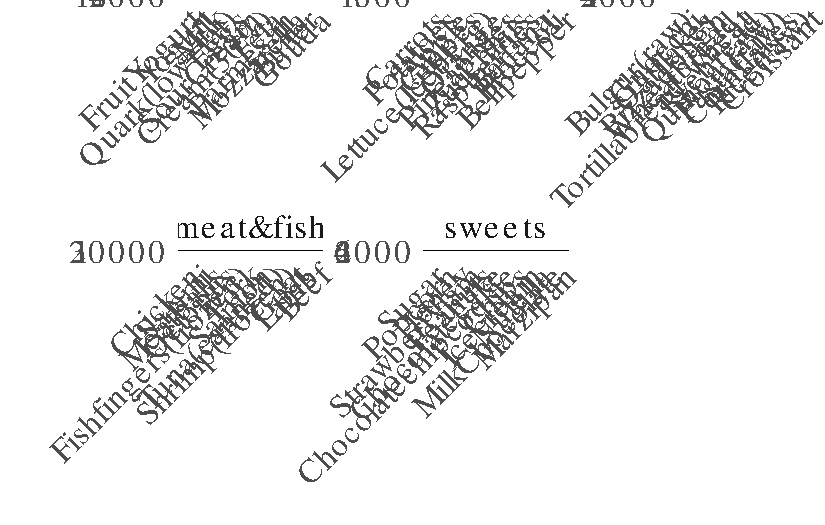
\includegraphics{items_files/figure-pdf/unnamed-chunk-6-1.pdf}

\subsection{Relative}

\begin{Shaded}
\begin{Highlighting}[]
\FunctionTok{ggplot}\NormalTok{(items,}\FunctionTok{aes}\NormalTok{(}\AttributeTok{x =} \FunctionTok{fct\_reorder}\NormalTok{(name,}\StringTok{\textasciigrave{}}\AttributeTok{g CO2 pro kg}\StringTok{\textasciigrave{}}\NormalTok{),}
                 \AttributeTok{y =} \StringTok{\textasciigrave{}}\AttributeTok{g CO2 pro kg}\StringTok{\textasciigrave{}}\NormalTok{,}
                 \AttributeTok{color =} \FunctionTok{factor}\NormalTok{(seeding\_CO2))) }\SpecialCharTok{+}
  \FunctionTok{geom\_point}\NormalTok{(}\AttributeTok{size=}\NormalTok{p\_size) }\SpecialCharTok{+}
  \FunctionTok{geom\_linerange}\NormalTok{(}\FunctionTok{aes}\NormalTok{(}\AttributeTok{ymax =} \StringTok{\textasciigrave{}}\AttributeTok{g CO2 pro kg}\StringTok{\textasciigrave{}}\NormalTok{, }\AttributeTok{ymin =} \DecValTok{0}\NormalTok{),}\AttributeTok{linewidth=}\NormalTok{lwd) }\SpecialCharTok{+}
  \FunctionTok{facet\_wrap}\NormalTok{(.}\SpecialCharTok{\textasciitilde{}}\NormalTok{category,}\AttributeTok{scales=}\StringTok{"free"}\NormalTok{,}\AttributeTok{nrow=}\DecValTok{2}\NormalTok{)}\SpecialCharTok{+}
  \FunctionTok{labs}\NormalTok{(}\AttributeTok{title =} \StringTok{""}\NormalTok{,}
       \AttributeTok{x     =} \StringTok{""}\NormalTok{,}
       \AttributeTok{y     =} \StringTok{""}\NormalTok{,}
       \AttributeTok{color =} \StringTok{"Seed Item"}\NormalTok{) }\SpecialCharTok{+}
  \FunctionTok{scale\_color\_manual}\NormalTok{(}\AttributeTok{values =} \FunctionTok{c}\NormalTok{(}\StringTok{"black"}\NormalTok{,}\StringTok{"\#22A884FF"}\NormalTok{)) }\SpecialCharTok{+}
  \FunctionTok{theme\_nice}\NormalTok{() }\SpecialCharTok{+}
  \FunctionTok{theme}\NormalTok{(}\AttributeTok{axis.text.x =} \FunctionTok{element\_text}\NormalTok{(}\AttributeTok{angle =} \DecValTok{45}\NormalTok{,}\AttributeTok{hjust =} \DecValTok{1}\NormalTok{)) }\SpecialCharTok{+}
  \FunctionTok{scale\_y\_continuous}\NormalTok{(}\AttributeTok{expand =} \FunctionTok{c}\NormalTok{(}\DecValTok{0}\NormalTok{, }\DecValTok{0}\NormalTok{), }\AttributeTok{limits =} \FunctionTok{c}\NormalTok{(}\DecValTok{0}\NormalTok{,}\DecValTok{28500}\NormalTok{))}
\end{Highlighting}
\end{Shaded}

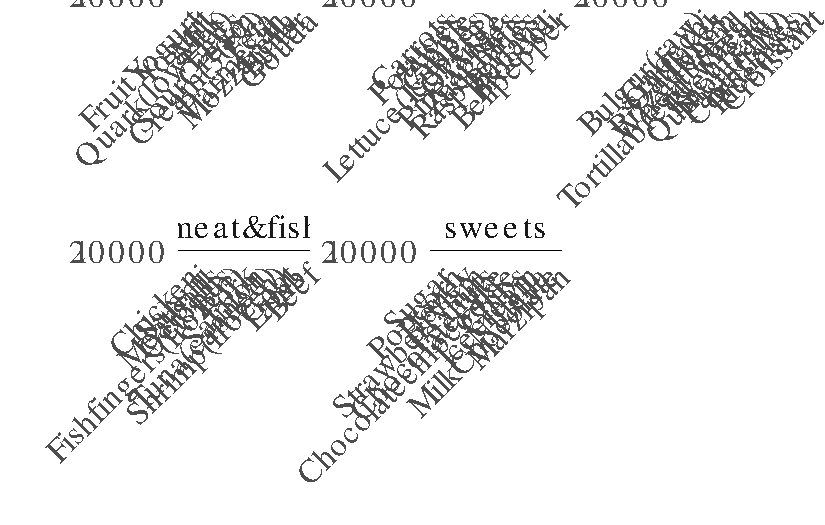
\includegraphics{items_files/figure-pdf/unnamed-chunk-7-1.pdf}

\subsection{Kcal per 100g}\label{kcal-per-100g}

\subsection{Overall}

\begin{Shaded}
\begin{Highlighting}[]
\FunctionTok{ggplot}\NormalTok{(items,}\FunctionTok{aes}\NormalTok{(}\AttributeTok{x =} \FunctionTok{fct\_reorder}\NormalTok{(name,}\StringTok{\textasciigrave{}}\AttributeTok{Kcal pro 100g}\StringTok{\textasciigrave{}}\NormalTok{),}
                 \AttributeTok{y =} \StringTok{\textasciigrave{}}\AttributeTok{Kcal pro 100g}\StringTok{\textasciigrave{}}\NormalTok{,}
                 \AttributeTok{color =} \FunctionTok{factor}\NormalTok{(seeding\_Kcal))) }\SpecialCharTok{+}
  \FunctionTok{geom\_point}\NormalTok{(}\AttributeTok{size=}\NormalTok{p\_size) }\SpecialCharTok{+}
  \FunctionTok{geom\_linerange}\NormalTok{(}\FunctionTok{aes}\NormalTok{(}\AttributeTok{ymax =} \StringTok{\textasciigrave{}}\AttributeTok{Kcal pro 100g}\StringTok{\textasciigrave{}}\NormalTok{, }\AttributeTok{ymin =} \DecValTok{0}\NormalTok{),}\AttributeTok{linewidth=}\NormalTok{lwd) }\SpecialCharTok{+}
  \FunctionTok{facet\_wrap}\NormalTok{(.}\SpecialCharTok{\textasciitilde{}}\NormalTok{category,}\AttributeTok{scales=}\StringTok{"free"}\NormalTok{,}\AttributeTok{nrow=}\DecValTok{2}\NormalTok{)}\SpecialCharTok{+}
  \FunctionTok{labs}\NormalTok{(}\AttributeTok{title =} \StringTok{""}\NormalTok{,}
       \AttributeTok{x     =} \StringTok{""}\NormalTok{,}
       \AttributeTok{y     =} \StringTok{""}\NormalTok{,}
       \AttributeTok{color =} \StringTok{"Seed Item"}\NormalTok{) }\SpecialCharTok{+}
  \FunctionTok{scale\_color\_manual}\NormalTok{(}\AttributeTok{values =} \FunctionTok{c}\NormalTok{(}\StringTok{"black"}\NormalTok{,}\StringTok{"\#22A884FF"}\NormalTok{)) }\SpecialCharTok{+}
  \FunctionTok{theme\_nice}\NormalTok{() }\SpecialCharTok{+}
  \FunctionTok{theme}\NormalTok{(}\AttributeTok{axis.text.x =} \FunctionTok{element\_text}\NormalTok{(}\AttributeTok{angle =} \DecValTok{45}\NormalTok{,}\AttributeTok{hjust =} \DecValTok{1}\NormalTok{)) }\SpecialCharTok{+}
  \FunctionTok{scale\_y\_continuous}\NormalTok{(}\FunctionTok{expansion}\NormalTok{(}\AttributeTok{mult =} \FunctionTok{c}\NormalTok{(}\DecValTok{0}\NormalTok{, }\FloatTok{0.2}\NormalTok{)))}
\end{Highlighting}
\end{Shaded}

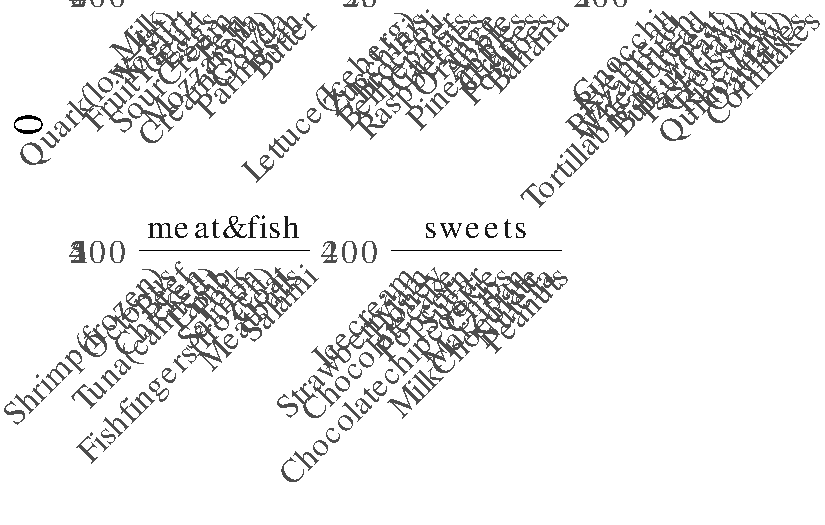
\includegraphics{items_files/figure-pdf/unnamed-chunk-8-1.pdf}

\subsection{Relative}

\begin{Shaded}
\begin{Highlighting}[]
\FunctionTok{ggplot}\NormalTok{(items,}\FunctionTok{aes}\NormalTok{(}\AttributeTok{x =} \FunctionTok{fct\_reorder}\NormalTok{(name,}\StringTok{\textasciigrave{}}\AttributeTok{Kcal pro 100g}\StringTok{\textasciigrave{}}\NormalTok{),}
                 \AttributeTok{y =} \StringTok{\textasciigrave{}}\AttributeTok{Kcal pro 100g}\StringTok{\textasciigrave{}}\NormalTok{,}
                 \AttributeTok{color =} \FunctionTok{factor}\NormalTok{(seeding\_Kcal))) }\SpecialCharTok{+}
  \FunctionTok{geom\_point}\NormalTok{(}\AttributeTok{size=}\NormalTok{p\_size) }\SpecialCharTok{+}
  \FunctionTok{geom\_linerange}\NormalTok{(}\FunctionTok{aes}\NormalTok{(}\AttributeTok{ymax =} \StringTok{\textasciigrave{}}\AttributeTok{Kcal pro 100g}\StringTok{\textasciigrave{}}\NormalTok{, }\AttributeTok{ymin =} \DecValTok{0}\NormalTok{),}\AttributeTok{linewidth=}\NormalTok{lwd) }\SpecialCharTok{+}
  \FunctionTok{facet\_wrap}\NormalTok{(.}\SpecialCharTok{\textasciitilde{}}\NormalTok{category,}\AttributeTok{scales=}\StringTok{"free"}\NormalTok{,}\AttributeTok{nrow=}\DecValTok{2}\NormalTok{)}\SpecialCharTok{+}
  \FunctionTok{labs}\NormalTok{(}\AttributeTok{title =} \StringTok{""}\NormalTok{,}
       \AttributeTok{x     =} \StringTok{""}\NormalTok{,}
       \AttributeTok{y     =} \StringTok{""}\NormalTok{,}
       \AttributeTok{color =} \StringTok{"Seed Item"}\NormalTok{) }\SpecialCharTok{+}
  \FunctionTok{scale\_color\_manual}\NormalTok{(}\AttributeTok{values =} \FunctionTok{c}\NormalTok{(}\StringTok{"black"}\NormalTok{,}\StringTok{"\#22A884FF"}\NormalTok{)) }\SpecialCharTok{+}
  \FunctionTok{theme\_nice}\NormalTok{() }\SpecialCharTok{+}
  \FunctionTok{theme}\NormalTok{(}\AttributeTok{axis.text.x =} \FunctionTok{element\_text}\NormalTok{(}\AttributeTok{angle =} \DecValTok{45}\NormalTok{,}\AttributeTok{hjust =} \DecValTok{1}\NormalTok{)) }\SpecialCharTok{+}
  \FunctionTok{scale\_y\_continuous}\NormalTok{(}\AttributeTok{expand =} \FunctionTok{c}\NormalTok{(}\DecValTok{0}\NormalTok{, }\DecValTok{0}\NormalTok{), }\AttributeTok{limits =} \FunctionTok{c}\NormalTok{(}\DecValTok{0}\NormalTok{,}\DecValTok{800}\NormalTok{))}
\end{Highlighting}
\end{Shaded}

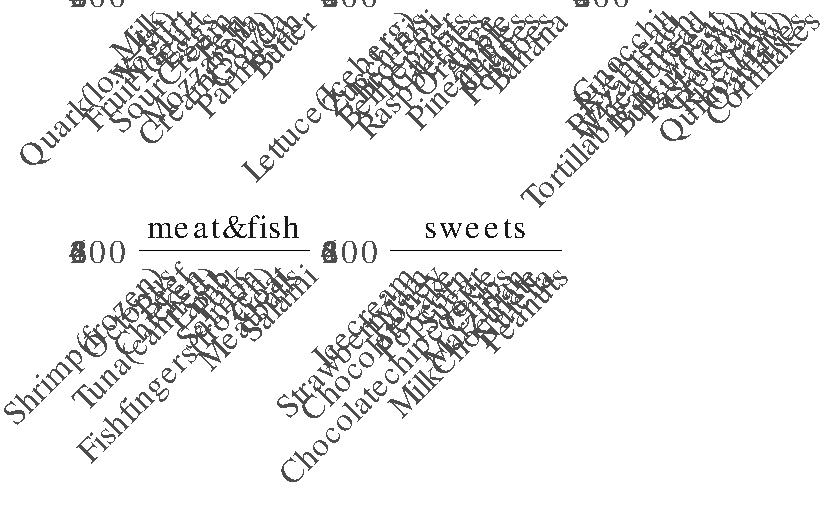
\includegraphics{items_files/figure-pdf/unnamed-chunk-9-1.pdf}



\end{document}
